%%%%%%%%%%% Resilient Kalman filter on the pruned safe sensor subset %%%%%%
In this section, the Kalman filter of Section~\ref{sec:system_model} is redesigned on the pruned safe support produced by Algorithm~\ref{Alg:ADL_AAG_P}, in order to maintain secure state estimation under FDIAs. The scheme is shown in Fig.~\ref{fig:resilient_L2_observer}: attack detection/localization returns an estimate $\hat{\mathcal{T}}^c$ of the safe sensors; pruning downselects the most trustworthy subset $\hat{\mathcal{T}}^c_{\eta}$; the resilient KF then updates using only $\mathbf{y}_{\hat{\mathcal{T}}^c_{\eta}}$, with the corresponding output matrix $C_{\hat{\mathcal{T}}^c_{\eta}}$ and noise covariance $R_{\hat{\mathcal{T}}^c_{\eta}}$.

\begin{figure}[h!]
    \centering
    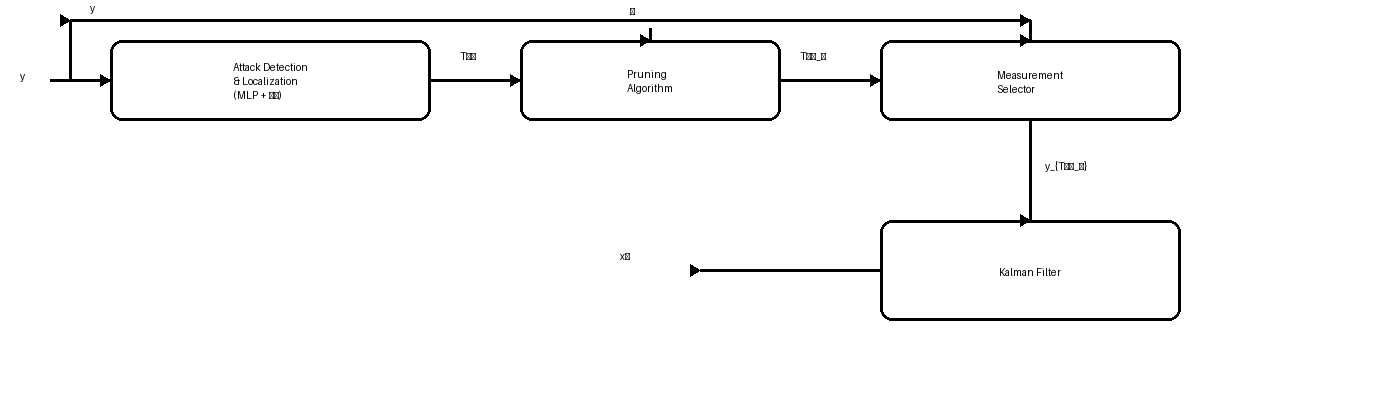
\includegraphics[width=\columnwidth]{image/resilient_L2_observer.png}
    \caption{Schematic diagram of the resilient Kalman filter with chi-square monitoring and support pruning}
    \label{fig:resilient_L2_observer}
\end{figure}

\subsection{Resilient Kalman filter}
Given $\hat{\mathcal{T}}^c_{\eta}$ at time $i$, the resilient KF uses the reduced measurement model
\begin{equation}\label{equ:reduced_meas}
\mathbf{y}_{\hat{\mathcal{T}}^c_{\eta},i}
=C_{\hat{\mathcal{T}}^c_{\eta}}\mathbf{x}_i+\mathbf{v}_{\hat{\mathcal{T}}^c_{\eta},i}+\mathbf{e}_{\hat{\mathcal{T}}^c_{\eta},i},
\end{equation}
and applies \eqref{equ:kf_predict}--\eqref{equ:kf_Pupdate} with $(C,R)$ replaced by $(C_{\hat{\mathcal{T}}^c_{\eta}},R_{\hat{\mathcal{T}}^c_{\eta}})$. Denote the resulting filtered estimate and covariance by $\hat{\mathbf{x}}_i'$ and $P_{i|i}(\hat{\mathcal{T}}^c_{\eta})$. By \eqref{equ:precision_after_pruning}, $\mathbf{e}_{\hat{\mathcal{T}}^c_{\eta},i}=\mathbf{0}$ with probability at least $\eta$.

When $|S|\ge k_0$ and $(A,C_S)$ is observable, the subset KF admits a unique stabilizing steady-state predicted covariance $P^-(S)\succ 0$ solving the DARE for $(A,C_S,Q,R_S)$, with filtered covariance
\begin{align}
P_{\infty}(S)&=(I-K(S)C_S)P^-(S), \label{equ:Pinf}\\
K(S)&=P^-(S)C_S^{\top}\big(C_SP^-(S)C_S^{\top}+R_S\big)^{-1}. \nonumber
\end{align}
The map $S\mapsto \mathrm{tr}\,P_{\infty}(S)$ is monotonically nonincreasing under set inclusion: if $S_1\subset S_2$ and both satisfy A2, then $\mathrm{tr}\,P_{\infty}(S_2)\le \mathrm{tr}\,P_{\infty}(S_1)$ \cite{anderson2012optimal}. This yields the graded estimation-error link in the sparsity--observability--precision chain.

\begin{theorem}[Resilient KF performance]\label{Thm:resilient_estimation_gaurentee}
Let $\hat{\mathcal{T}}^c_{\eta}$ be given by \eqref{equ:pruning_alg}, and suppose $\eta$ satisfies \eqref{equ:eta_upper_bound} with the localization performance criterion \eqref{equ:localization_performance_criterion}. Then, with probability at least $\eta$,
\begin{enumerate}
\item[(i)] $\mathbf{e}_{\hat{\mathcal{T}}^c_{\eta}}=\mathbf{0}$ and $|\hat{\mathcal{T}}^c_{\eta}|\ge k_0$, so $(A,C_{\hat{\mathcal{T}}^c_{\eta}})$ is observable;
\item[(ii)] the resilient KF coincides with the attack-free KF on the same sensor subset, and its steady-state mean-square error satisfies
\begin{equation}\label{equ:error_bound}
\lim_{i\to\infty}\mathbb{E}\big\|\hat{\mathbf{x}}_i'-\mathbf{x}_i\big\|_2^2
=\mathrm{tr}\,P_{\infty}(\hat{\mathcal{T}}^c_{\eta});
\end{equation}
\item[(iii)] relative to the full-sensor attack-free KF,
\begin{equation}\label{equ:error_gap}
\mathrm{tr}\,P_{\infty}(\{1,\ldots,m\})
\le
\mathrm{tr}\,P_{\infty}(\hat{\mathcal{T}}^c_{\eta})
\le
\mathrm{tr}\,P_{\infty}(S_{k_0}),
\end{equation}
for every observable subset $S_{k_0}$ of size $k_0$ that can arise from pruning at reliability $\eta$.
\end{enumerate}
\end{theorem}
\begin{proof}
Claim~(i) follows from \eqref{equ:precision_after_pruning}, Theorem~\ref{Thm:eta_upper_bound}, and assumption~A2. On that event the reduced measurements equal the attack-free subset measurements, so the KF recursions---and hence the limiting covariance \eqref{equ:Pinf}---coincide with the attack-free subset filter, which is claim~(ii). Claim~(iii) is the standard information monotonicity of the Riccati map under additional measurements, together with the worst-case size-$k_0$ subset admitted by the pruning length constraint.
\end{proof}

\begin{corollary}[Bridge summary]\label{Cor:bridge}
For attack sparsity $k$, observability threshold $k_0$, and localization confidences $\{\mathbf{p}_i\}$, Propositions~\ref{Prop:sparsity_observability}--\ref{Prop:precision_observability} and Theorem~\ref{Thm:resilient_estimation_gaurentee} jointly imply: every $\eta\in(0,\eta^{\star}]$ yields a pruned set that is clean and observable with probability $\ge\eta$, and the KF error is then exactly $\mathrm{tr}\,P_{\infty}(\hat{\mathcal{T}}^c_{\eta})$, sandwiched between the full-sensor and worst $k_0$-sensor Riccati costs. Thus sparsity constrains feasible $(k,k_0)$, precision $\eta$ trades against set size (hence against $\mathrm{tr}\,P_{\infty}$), and estimation error is quantitatively tied to both.
\end{corollary}

The chi-square monitor \eqref{equ:chisq_detector} may still be evaluated on the innovation of the resilient KF (with $S_i$ computed from $C_{\hat{\mathcal{T}}^c_{\eta}}$) to provide an online global alarm, while the MLP+pruning path supplies the channel support required by \eqref{equ:error_bound}--\eqref{equ:error_gap}.
